\documentclass[12pt,a4paper]{article}

\usepackage[a4paper,width=160mm,top=25mm,bottom=25mm]{geometry}

\usepackage{fancyhdr}
\pagestyle{fancy}
\fancyhf{}
\fancyhead[EL]{\nouppercase\leftmark}
\fancyhead[OR]{\nouppercase\rightmark}
\fancyhead[ER,OL]{\thepage}

\usepackage{url}
\usepackage[hidelinks]{hyperref}

\renewcommand{\linethickness}{0.05em}
\usepackage[brazil]{babel}   
\usepackage{titlesec}
\newcommand{\sectionbreak}{\clearpage}


\title{Processando a Informação: um livro prático de programação independente de linguagem 
\\\large\vspace{2cm}
Rogério Perino de Oliveira Neves 
\\\vspace{5mm}
Francisco de Assis Zampirolli
\\\large\vspace{2cm}
EDUFABC
\\ \url{editora.ufabc.edu.br}
\\\Huge\vspace{3cm}
Notas de Aulas inspiradas no livro
\\\Large\vspace{1cm}
Utilizando a(s) Linguagem(ns) de Programação: 
\\\Huge\vspace{1cm}
C
\\\large\vspace{1cm}
Exemplos adaptados para Correção Automática no Moodle+VPL
\vspace{2cm}}
\author{Francisco de Assis Zampirolli\vspace{1cm}}


    \usepackage[breakable]{tcolorbox}
    \usepackage{parskip} % Stop auto-indenting (to mimic markdown behaviour)
    

    % Basic figure setup, for now with no caption control since it's done
    % automatically by Pandoc (which extracts ![](path) syntax from Markdown).
    \usepackage{graphicx}
    % Maintain compatibility with old templates. Remove in nbconvert 6.0
    \let\Oldincludegraphics\includegraphics
    % Ensure that by default, figures have no caption (until we provide a
    % proper Figure object with a Caption API and a way to capture that
    % in the conversion process - todo).
    \usepackage{caption}
    \DeclareCaptionFormat{nocaption}{}
    \captionsetup{format=nocaption,aboveskip=0pt,belowskip=0pt}

    \usepackage{float}
    \floatplacement{figure}{H} % forces figures to be placed at the correct location
    \usepackage{xcolor} % Allow colors to be defined
    \usepackage{enumerate} % Needed for markdown enumerations to work
    \usepackage{geometry} % Used to adjust the document margins
    \usepackage{amsmath} % Equations
    \usepackage{amssymb} % Equations
    \usepackage{textcomp} % defines textquotesingle
    % Hack from http://tex.stackexchange.com/a/47451/13684:
    \AtBeginDocument{%
        \def\PYZsq{\textquotesingle}% Upright quotes in Pygmentized code
    }
    \usepackage{upquote} % Upright quotes for verbatim code
    \usepackage{eurosym} % defines \euro

    \usepackage{iftex}
    \ifPDFTeX
        \usepackage[T1]{fontenc}
        \IfFileExists{alphabeta.sty}{
              \usepackage{alphabeta}
          }{
              \usepackage[mathletters]{ucs}
              \usepackage[utf8x]{inputenc}
          }
    \else
        \usepackage{fontspec}
        \usepackage{unicode-math}
    \fi

    \usepackage{fancyvrb} % verbatim replacement that allows latex
    \usepackage{grffile} % extends the file name processing of package graphics 
                         % to support a larger range
    \makeatletter % fix for old versions of grffile with XeLaTeX
    \@ifpackagelater{grffile}{2019/11/01}
    {
      % Do nothing on new versions
    }
    {
      \def\Gread@@xetex#1{%
        \IfFileExists{"\Gin@base".bb}%
        {\Gread@eps{\Gin@base.bb}}%
        {\Gread@@xetex@aux#1}%
      }
    }
    \makeatother
    \usepackage[Export]{adjustbox} % Used to constrain images to a maximum size
    \adjustboxset{max size={0.9\linewidth}{0.9\paperheight}}

    % The hyperref package gives us a pdf with properly built
    % internal navigation ('pdf bookmarks' for the table of contents,
    % internal cross-reference links, web links for URLs, etc.)
    \usepackage{hyperref}
    % The default LaTeX title has an obnoxious amount of whitespace. By default,
    % titling removes some of it. It also provides customization options.
    \usepackage{titling}
    \usepackage{longtable} % longtable support required by pandoc >1.10
    \usepackage{booktabs}  % table support for pandoc > 1.12.2
    \usepackage{array}     % table support for pandoc >= 2.11.3
    \usepackage{calc}      % table minipage width calculation for pandoc >= 2.11.1
    \usepackage[inline]{enumitem} % IRkernel/repr support (it uses the enumerate* environment)
    \usepackage[normalem]{ulem} % ulem is needed to support strikethroughs (\sout)
                                % normalem makes italics be italics, not underlines
    \usepackage{mathrsfs}
    

    
    % Colors for the hyperref package
    \definecolor{urlcolor}{rgb}{0,.145,.698}
    \definecolor{linkcolor}{rgb}{.71,0.21,0.01}
    \definecolor{citecolor}{rgb}{.12,.54,.11}

    % ANSI colors
    \definecolor{ansi-black}{HTML}{3E424D}
    \definecolor{ansi-black-intense}{HTML}{282C36}
    \definecolor{ansi-red}{HTML}{E75C58}
    \definecolor{ansi-red-intense}{HTML}{B22B31}
    \definecolor{ansi-green}{HTML}{00A250}
    \definecolor{ansi-green-intense}{HTML}{007427}
    \definecolor{ansi-yellow}{HTML}{DDB62B}
    \definecolor{ansi-yellow-intense}{HTML}{B27D12}
    \definecolor{ansi-blue}{HTML}{208FFB}
    \definecolor{ansi-blue-intense}{HTML}{0065CA}
    \definecolor{ansi-magenta}{HTML}{D160C4}
    \definecolor{ansi-magenta-intense}{HTML}{A03196}
    \definecolor{ansi-cyan}{HTML}{60C6C8}
    \definecolor{ansi-cyan-intense}{HTML}{258F8F}
    \definecolor{ansi-white}{HTML}{C5C1B4}
    \definecolor{ansi-white-intense}{HTML}{A1A6B2}
    \definecolor{ansi-default-inverse-fg}{HTML}{FFFFFF}
    \definecolor{ansi-default-inverse-bg}{HTML}{000000}

    % common color for the border for error outputs.
    \definecolor{outerrorbackground}{HTML}{FFDFDF}

    % commands and environments needed by pandoc snippets
    % extracted from the output of `pandoc -s`
    \providecommand{\tightlist}{%
      \setlength{\itemsep}{0pt}\setlength{\parskip}{0pt}}
    \DefineVerbatimEnvironment{Highlighting}{Verbatim}{commandchars=\\\{\}}
    % Add ',fontsize=\small' for more characters per line
    \newenvironment{Shaded}{}{}
    \newcommand{\KeywordTok}[1]{\textcolor[rgb]{0.00,0.44,0.13}{\textbf{{#1}}}}
    \newcommand{\DataTypeTok}[1]{\textcolor[rgb]{0.56,0.13,0.00}{{#1}}}
    \newcommand{\DecValTok}[1]{\textcolor[rgb]{0.25,0.63,0.44}{{#1}}}
    \newcommand{\BaseNTok}[1]{\textcolor[rgb]{0.25,0.63,0.44}{{#1}}}
    \newcommand{\FloatTok}[1]{\textcolor[rgb]{0.25,0.63,0.44}{{#1}}}
    \newcommand{\CharTok}[1]{\textcolor[rgb]{0.25,0.44,0.63}{{#1}}}
    \newcommand{\StringTok}[1]{\textcolor[rgb]{0.25,0.44,0.63}{{#1}}}
    \newcommand{\CommentTok}[1]{\textcolor[rgb]{0.38,0.63,0.69}{\textit{{#1}}}}
    \newcommand{\OtherTok}[1]{\textcolor[rgb]{0.00,0.44,0.13}{{#1}}}
    \newcommand{\AlertTok}[1]{\textcolor[rgb]{1.00,0.00,0.00}{\textbf{{#1}}}}
    \newcommand{\FunctionTok}[1]{\textcolor[rgb]{0.02,0.16,0.49}{{#1}}}
    \newcommand{\RegionMarkerTok}[1]{{#1}}
    \newcommand{\ErrorTok}[1]{\textcolor[rgb]{1.00,0.00,0.00}{\textbf{{#1}}}}
    \newcommand{\NormalTok}[1]{{#1}}
    
    % Additional commands for more recent versions of Pandoc
    \newcommand{\ConstantTok}[1]{\textcolor[rgb]{0.53,0.00,0.00}{{#1}}}
    \newcommand{\SpecialCharTok}[1]{\textcolor[rgb]{0.25,0.44,0.63}{{#1}}}
    \newcommand{\VerbatimStringTok}[1]{\textcolor[rgb]{0.25,0.44,0.63}{{#1}}}
    \newcommand{\SpecialStringTok}[1]{\textcolor[rgb]{0.73,0.40,0.53}{{#1}}}
    \newcommand{\ImportTok}[1]{{#1}}
    \newcommand{\DocumentationTok}[1]{\textcolor[rgb]{0.73,0.13,0.13}{\textit{{#1}}}}
    \newcommand{\AnnotationTok}[1]{\textcolor[rgb]{0.38,0.63,0.69}{\textbf{\textit{{#1}}}}}
    \newcommand{\CommentVarTok}[1]{\textcolor[rgb]{0.38,0.63,0.69}{\textbf{\textit{{#1}}}}}
    \newcommand{\VariableTok}[1]{\textcolor[rgb]{0.10,0.09,0.49}{{#1}}}
    \newcommand{\ControlFlowTok}[1]{\textcolor[rgb]{0.00,0.44,0.13}{\textbf{{#1}}}}
    \newcommand{\OperatorTok}[1]{\textcolor[rgb]{0.40,0.40,0.40}{{#1}}}
    \newcommand{\BuiltInTok}[1]{{#1}}
    \newcommand{\ExtensionTok}[1]{{#1}}
    \newcommand{\PreprocessorTok}[1]{\textcolor[rgb]{0.74,0.48,0.00}{{#1}}}
    \newcommand{\AttributeTok}[1]{\textcolor[rgb]{0.49,0.56,0.16}{{#1}}}
    \newcommand{\InformationTok}[1]{\textcolor[rgb]{0.38,0.63,0.69}{\textbf{\textit{{#1}}}}}
    \newcommand{\WarningTok}[1]{\textcolor[rgb]{0.38,0.63,0.69}{\textbf{\textit{{#1}}}}}
    
    
    % Define a nice break command that doesn't care if a line doesn't already
    % exist.
    \def\br{\hspace*{\fill} \\* }
    % Math Jax compatibility definitions
    \def\gt{>}
    \def\lt{<}
    \let\Oldtex\TeX
    \let\Oldlatex\LaTeX
    \renewcommand{\TeX}{\textrm{\Oldtex}}
    \renewcommand{\LaTeX}{\textrm{\Oldlatex}}
    % Document parameters
    % Document title
    %\title{cap2.part1.c}
    
    
    
    
    
% Pygments definitions
\makeatletter
\def\PY@reset{\let\PY@it=\relax \let\PY@bf=\relax%
    \let\PY@ul=\relax \let\PY@tc=\relax%
    \let\PY@bc=\relax \let\PY@ff=\relax}
\def\PY@tok#1{\csname PY@tok@#1\endcsname}
\def\PY@toks#1+{\ifx\relax#1\empty\else%
    \PY@tok{#1}\expandafter\PY@toks\fi}
\def\PY@do#1{\PY@bc{\PY@tc{\PY@ul{%
    \PY@it{\PY@bf{\PY@ff{#1}}}}}}}
\def\PY#1#2{\PY@reset\PY@toks#1+\relax+\PY@do{#2}}

\@namedef{PY@tok@w}{\def\PY@tc##1{\textcolor[rgb]{0.73,0.73,0.73}{##1}}}
\@namedef{PY@tok@c}{\let\PY@it=\textit\def\PY@tc##1{\textcolor[rgb]{0.24,0.48,0.48}{##1}}}
\@namedef{PY@tok@cp}{\def\PY@tc##1{\textcolor[rgb]{0.61,0.40,0.00}{##1}}}
\@namedef{PY@tok@k}{\let\PY@bf=\textbf\def\PY@tc##1{\textcolor[rgb]{0.00,0.50,0.00}{##1}}}
\@namedef{PY@tok@kp}{\def\PY@tc##1{\textcolor[rgb]{0.00,0.50,0.00}{##1}}}
\@namedef{PY@tok@kt}{\def\PY@tc##1{\textcolor[rgb]{0.69,0.00,0.25}{##1}}}
\@namedef{PY@tok@o}{\def\PY@tc##1{\textcolor[rgb]{0.40,0.40,0.40}{##1}}}
\@namedef{PY@tok@ow}{\let\PY@bf=\textbf\def\PY@tc##1{\textcolor[rgb]{0.67,0.13,1.00}{##1}}}
\@namedef{PY@tok@nb}{\def\PY@tc##1{\textcolor[rgb]{0.00,0.50,0.00}{##1}}}
\@namedef{PY@tok@nf}{\def\PY@tc##1{\textcolor[rgb]{0.00,0.00,1.00}{##1}}}
\@namedef{PY@tok@nc}{\let\PY@bf=\textbf\def\PY@tc##1{\textcolor[rgb]{0.00,0.00,1.00}{##1}}}
\@namedef{PY@tok@nn}{\let\PY@bf=\textbf\def\PY@tc##1{\textcolor[rgb]{0.00,0.00,1.00}{##1}}}
\@namedef{PY@tok@ne}{\let\PY@bf=\textbf\def\PY@tc##1{\textcolor[rgb]{0.80,0.25,0.22}{##1}}}
\@namedef{PY@tok@nv}{\def\PY@tc##1{\textcolor[rgb]{0.10,0.09,0.49}{##1}}}
\@namedef{PY@tok@no}{\def\PY@tc##1{\textcolor[rgb]{0.53,0.00,0.00}{##1}}}
\@namedef{PY@tok@nl}{\def\PY@tc##1{\textcolor[rgb]{0.46,0.46,0.00}{##1}}}
\@namedef{PY@tok@ni}{\let\PY@bf=\textbf\def\PY@tc##1{\textcolor[rgb]{0.44,0.44,0.44}{##1}}}
\@namedef{PY@tok@na}{\def\PY@tc##1{\textcolor[rgb]{0.41,0.47,0.13}{##1}}}
\@namedef{PY@tok@nt}{\let\PY@bf=\textbf\def\PY@tc##1{\textcolor[rgb]{0.00,0.50,0.00}{##1}}}
\@namedef{PY@tok@nd}{\def\PY@tc##1{\textcolor[rgb]{0.67,0.13,1.00}{##1}}}
\@namedef{PY@tok@s}{\def\PY@tc##1{\textcolor[rgb]{0.73,0.13,0.13}{##1}}}
\@namedef{PY@tok@sd}{\let\PY@it=\textit\def\PY@tc##1{\textcolor[rgb]{0.73,0.13,0.13}{##1}}}
\@namedef{PY@tok@si}{\let\PY@bf=\textbf\def\PY@tc##1{\textcolor[rgb]{0.64,0.35,0.47}{##1}}}
\@namedef{PY@tok@se}{\let\PY@bf=\textbf\def\PY@tc##1{\textcolor[rgb]{0.67,0.36,0.12}{##1}}}
\@namedef{PY@tok@sr}{\def\PY@tc##1{\textcolor[rgb]{0.64,0.35,0.47}{##1}}}
\@namedef{PY@tok@ss}{\def\PY@tc##1{\textcolor[rgb]{0.10,0.09,0.49}{##1}}}
\@namedef{PY@tok@sx}{\def\PY@tc##1{\textcolor[rgb]{0.00,0.50,0.00}{##1}}}
\@namedef{PY@tok@m}{\def\PY@tc##1{\textcolor[rgb]{0.40,0.40,0.40}{##1}}}
\@namedef{PY@tok@gh}{\let\PY@bf=\textbf\def\PY@tc##1{\textcolor[rgb]{0.00,0.00,0.50}{##1}}}
\@namedef{PY@tok@gu}{\let\PY@bf=\textbf\def\PY@tc##1{\textcolor[rgb]{0.50,0.00,0.50}{##1}}}
\@namedef{PY@tok@gd}{\def\PY@tc##1{\textcolor[rgb]{0.63,0.00,0.00}{##1}}}
\@namedef{PY@tok@gi}{\def\PY@tc##1{\textcolor[rgb]{0.00,0.52,0.00}{##1}}}
\@namedef{PY@tok@gr}{\def\PY@tc##1{\textcolor[rgb]{0.89,0.00,0.00}{##1}}}
\@namedef{PY@tok@ge}{\let\PY@it=\textit}
\@namedef{PY@tok@gs}{\let\PY@bf=\textbf}
\@namedef{PY@tok@gp}{\let\PY@bf=\textbf\def\PY@tc##1{\textcolor[rgb]{0.00,0.00,0.50}{##1}}}
\@namedef{PY@tok@go}{\def\PY@tc##1{\textcolor[rgb]{0.44,0.44,0.44}{##1}}}
\@namedef{PY@tok@gt}{\def\PY@tc##1{\textcolor[rgb]{0.00,0.27,0.87}{##1}}}
\@namedef{PY@tok@err}{\def\PY@bc##1{{\setlength{\fboxsep}{\string -\fboxrule}\fcolorbox[rgb]{1.00,0.00,0.00}{1,1,1}{\strut ##1}}}}
\@namedef{PY@tok@kc}{\let\PY@bf=\textbf\def\PY@tc##1{\textcolor[rgb]{0.00,0.50,0.00}{##1}}}
\@namedef{PY@tok@kd}{\let\PY@bf=\textbf\def\PY@tc##1{\textcolor[rgb]{0.00,0.50,0.00}{##1}}}
\@namedef{PY@tok@kn}{\let\PY@bf=\textbf\def\PY@tc##1{\textcolor[rgb]{0.00,0.50,0.00}{##1}}}
\@namedef{PY@tok@kr}{\let\PY@bf=\textbf\def\PY@tc##1{\textcolor[rgb]{0.00,0.50,0.00}{##1}}}
\@namedef{PY@tok@bp}{\def\PY@tc##1{\textcolor[rgb]{0.00,0.50,0.00}{##1}}}
\@namedef{PY@tok@fm}{\def\PY@tc##1{\textcolor[rgb]{0.00,0.00,1.00}{##1}}}
\@namedef{PY@tok@vc}{\def\PY@tc##1{\textcolor[rgb]{0.10,0.09,0.49}{##1}}}
\@namedef{PY@tok@vg}{\def\PY@tc##1{\textcolor[rgb]{0.10,0.09,0.49}{##1}}}
\@namedef{PY@tok@vi}{\def\PY@tc##1{\textcolor[rgb]{0.10,0.09,0.49}{##1}}}
\@namedef{PY@tok@vm}{\def\PY@tc##1{\textcolor[rgb]{0.10,0.09,0.49}{##1}}}
\@namedef{PY@tok@sa}{\def\PY@tc##1{\textcolor[rgb]{0.73,0.13,0.13}{##1}}}
\@namedef{PY@tok@sb}{\def\PY@tc##1{\textcolor[rgb]{0.73,0.13,0.13}{##1}}}
\@namedef{PY@tok@sc}{\def\PY@tc##1{\textcolor[rgb]{0.73,0.13,0.13}{##1}}}
\@namedef{PY@tok@dl}{\def\PY@tc##1{\textcolor[rgb]{0.73,0.13,0.13}{##1}}}
\@namedef{PY@tok@s2}{\def\PY@tc##1{\textcolor[rgb]{0.73,0.13,0.13}{##1}}}
\@namedef{PY@tok@sh}{\def\PY@tc##1{\textcolor[rgb]{0.73,0.13,0.13}{##1}}}
\@namedef{PY@tok@s1}{\def\PY@tc##1{\textcolor[rgb]{0.73,0.13,0.13}{##1}}}
\@namedef{PY@tok@mb}{\def\PY@tc##1{\textcolor[rgb]{0.40,0.40,0.40}{##1}}}
\@namedef{PY@tok@mf}{\def\PY@tc##1{\textcolor[rgb]{0.40,0.40,0.40}{##1}}}
\@namedef{PY@tok@mh}{\def\PY@tc##1{\textcolor[rgb]{0.40,0.40,0.40}{##1}}}
\@namedef{PY@tok@mi}{\def\PY@tc##1{\textcolor[rgb]{0.40,0.40,0.40}{##1}}}
\@namedef{PY@tok@il}{\def\PY@tc##1{\textcolor[rgb]{0.40,0.40,0.40}{##1}}}
\@namedef{PY@tok@mo}{\def\PY@tc##1{\textcolor[rgb]{0.40,0.40,0.40}{##1}}}
\@namedef{PY@tok@ch}{\let\PY@it=\textit\def\PY@tc##1{\textcolor[rgb]{0.24,0.48,0.48}{##1}}}
\@namedef{PY@tok@cm}{\let\PY@it=\textit\def\PY@tc##1{\textcolor[rgb]{0.24,0.48,0.48}{##1}}}
\@namedef{PY@tok@cpf}{\let\PY@it=\textit\def\PY@tc##1{\textcolor[rgb]{0.24,0.48,0.48}{##1}}}
\@namedef{PY@tok@c1}{\let\PY@it=\textit\def\PY@tc##1{\textcolor[rgb]{0.24,0.48,0.48}{##1}}}
\@namedef{PY@tok@cs}{\let\PY@it=\textit\def\PY@tc##1{\textcolor[rgb]{0.24,0.48,0.48}{##1}}}

\def\PYZbs{\char`\\}
\def\PYZus{\char`\_}
\def\PYZob{\char`\{}
\def\PYZcb{\char`\}}
\def\PYZca{\char`\^}
\def\PYZam{\char`\&}
\def\PYZlt{\char`\<}
\def\PYZgt{\char`\>}
\def\PYZsh{\char`\#}
\def\PYZpc{\char`\%}
\def\PYZdl{\char`\$}
\def\PYZhy{\char`\-}
\def\PYZsq{\char`\'}
\def\PYZdq{\char`\"}
\def\PYZti{\char`\~}
% for compatibility with earlier versions
\def\PYZat{@}
\def\PYZlb{[}
\def\PYZrb{]}
\makeatother


    % For linebreaks inside Verbatim environment from package fancyvrb. 
    \makeatletter
        \newbox\Wrappedcontinuationbox 
        \newbox\Wrappedvisiblespacebox 
        \newcommand*\Wrappedvisiblespace {\textcolor{red}{\textvisiblespace}} 
        \newcommand*\Wrappedcontinuationsymbol {\textcolor{red}{\llap{\tiny$\m@th\hookrightarrow$}}} 
        \newcommand*\Wrappedcontinuationindent {3ex } 
        \newcommand*\Wrappedafterbreak {\kern\Wrappedcontinuationindent\copy\Wrappedcontinuationbox} 
        % Take advantage of the already applied Pygments mark-up to insert 
        % potential linebreaks for TeX processing. 
        %        {, <, #, %, $, ' and ": go to next line. 
        %        _, }, ^, &, >, - and ~: stay at end of broken line. 
        % Use of \textquotesingle for straight quote. 
        \newcommand*\Wrappedbreaksatspecials {% 
            \def\PYGZus{\discretionary{\char`\_}{\Wrappedafterbreak}{\char`\_}}% 
            \def\PYGZob{\discretionary{}{\Wrappedafterbreak\char`\{}{\char`\{}}% 
            \def\PYGZcb{\discretionary{\char`\}}{\Wrappedafterbreak}{\char`\}}}% 
            \def\PYGZca{\discretionary{\char`\^}{\Wrappedafterbreak}{\char`\^}}% 
            \def\PYGZam{\discretionary{\char`\&}{\Wrappedafterbreak}{\char`\&}}% 
            \def\PYGZlt{\discretionary{}{\Wrappedafterbreak\char`\<}{\char`\<}}% 
            \def\PYGZgt{\discretionary{\char`\>}{\Wrappedafterbreak}{\char`\>}}% 
            \def\PYGZsh{\discretionary{}{\Wrappedafterbreak\char`\#}{\char`\#}}% 
            \def\PYGZpc{\discretionary{}{\Wrappedafterbreak\char`\%}{\char`\%}}% 
            \def\PYGZdl{\discretionary{}{\Wrappedafterbreak\char`\$}{\char`\$}}% 
            \def\PYGZhy{\discretionary{\char`\-}{\Wrappedafterbreak}{\char`\-}}% 
            \def\PYGZsq{\discretionary{}{\Wrappedafterbreak\textquotesingle}{\textquotesingle}}% 
            \def\PYGZdq{\discretionary{}{\Wrappedafterbreak\char`\"}{\char`\"}}% 
            \def\PYGZti{\discretionary{\char`\~}{\Wrappedafterbreak}{\char`\~}}% 
        } 
        % Some characters . , ; ? ! / are not pygmentized. 
        % This macro makes them "active" and they will insert potential linebreaks 
        \newcommand*\Wrappedbreaksatpunct {% 
            \lccode`\~`\.\lowercase{\def~}{\discretionary{\hbox{\char`\.}}{\Wrappedafterbreak}{\hbox{\char`\.}}}% 
            \lccode`\~`\,\lowercase{\def~}{\discretionary{\hbox{\char`\,}}{\Wrappedafterbreak}{\hbox{\char`\,}}}% 
            \lccode`\~`\;\lowercase{\def~}{\discretionary{\hbox{\char`\;}}{\Wrappedafterbreak}{\hbox{\char`\;}}}% 
            \lccode`\~`\:\lowercase{\def~}{\discretionary{\hbox{\char`\:}}{\Wrappedafterbreak}{\hbox{\char`\:}}}% 
            \lccode`\~`\?\lowercase{\def~}{\discretionary{\hbox{\char`\?}}{\Wrappedafterbreak}{\hbox{\char`\?}}}% 
            \lccode`\~`\!\lowercase{\def~}{\discretionary{\hbox{\char`\!}}{\Wrappedafterbreak}{\hbox{\char`\!}}}% 
            \lccode`\~`\/\lowercase{\def~}{\discretionary{\hbox{\char`\/}}{\Wrappedafterbreak}{\hbox{\char`\/}}}% 
            \catcode`\.\active
            \catcode`\,\active 
            \catcode`\;\active
            \catcode`\:\active
            \catcode`\?\active
            \catcode`\!\active
            \catcode`\/\active 
            \lccode`\~`\~ 	
        }
    \makeatother

    \let\OriginalVerbatim=\Verbatim
    \makeatletter
    \renewcommand{\Verbatim}[1][1]{%
        %\parskip\z@skip
        \sbox\Wrappedcontinuationbox {\Wrappedcontinuationsymbol}%
        \sbox\Wrappedvisiblespacebox {\FV@SetupFont\Wrappedvisiblespace}%
        \def\FancyVerbFormatLine ##1{\hsize\linewidth
            \vtop{\raggedright\hyphenpenalty\z@\exhyphenpenalty\z@
                \doublehyphendemerits\z@\finalhyphendemerits\z@
                \strut ##1\strut}%
        }%
        % If the linebreak is at a space, the latter will be displayed as visible
        % space at end of first line, and a continuation symbol starts next line.
        % Stretch/shrink are however usually zero for typewriter font.
        \def\FV@Space {%
            \nobreak\hskip\z@ plus\fontdimen3\font minus\fontdimen4\font
            \discretionary{\copy\Wrappedvisiblespacebox}{\Wrappedafterbreak}
            {\kern\fontdimen2\font}%
        }%
        
        % Allow breaks at special characters using \PYG... macros.
        \Wrappedbreaksatspecials
        % Breaks at punctuation characters . , ; ? ! and / need catcode=\active 	
        \OriginalVerbatim[#1,codes*=\Wrappedbreaksatpunct]%
    }
    \makeatother

    % Exact colors from NB
    \definecolor{incolor}{HTML}{303F9F}
    \definecolor{outcolor}{HTML}{D84315}
    \definecolor{cellborder}{HTML}{CFCFCF}
    \definecolor{cellbackground}{HTML}{F7F7F7}
    
    % prompt
    \makeatletter
    \newcommand{\boxspacing}{\kern\kvtcb@left@rule\kern\kvtcb@boxsep}
    \makeatother
    \newcommand{\prompt}[4]{
        {\ttfamily\llap{{\color{#2}[#3]:\hspace{3pt}#4}}\vspace{-\baselineskip}}
    }
    

    
    % Prevent overflowing lines due to hard-to-break entities
    \sloppy 
    % Setup hyperref package
    \hypersetup{
      breaklinks=true,  % so long urls are correctly broken across lines
      colorlinks=true,
      urlcolor=urlcolor,
      linkcolor=linkcolor,
      citecolor=citecolor,
      }
    % Slightly bigger margins than the latex defaults
    
    \geometry{verbose,tmargin=1in,bmargin=1in,lmargin=1in,rmargin=1in}
    
    

\begin{document}
    
    
\clearpage\maketitle
\thispagestyle{empty}
\tableofcontents

    
    

    
    \hypertarget{processando-a-informauxe7uxe3o-cap.-2-organizauxe7uxe3o-de-cuxf3digo}{%
\section{Processando a Informação: Cap. 2: Organização de
código}\label{processando-a-informauxe7uxe3o-cap.-2-organizauxe7uxe3o-de-cuxf3digo}}

    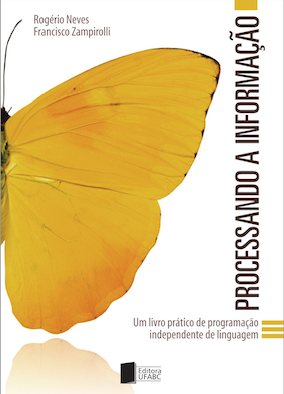
\includegraphics{"figs/Capa_Processando_Informacao.jpg"}

Este caderno (Notebook) é parte complementar \emph{online} do livro
\textbf{\href{https://editora.ufabc.edu.br/matematica-e-ciencias-da-computacao/58-processando-a-informacao}{Processando
a Informação}: um livro prático de programação independente de
linguagem}, que deve ser consultado no caso de dúvidas sobre os temas
apresentados.

\begin{quote}
Este conteúdo pode ser copiado e alterado livremente e foi inspirado
nesse livro.
\end{quote}

    \hypertarget{sumuxe1rio}{%
\subsection{Sumário}\label{sumuxe1rio}}

\begin{itemize}
\tightlist
\item
  Revisão do capítulo anterior
\item
  Programas sequenciais
\item
  Comentários
\item
  Desvios de fluxo
\item
  Programas e Subprogramas
\item
  Funções, métodos e modularização
\item
  Reaproveitamento e manutenção de código
\item
  Revisão deste capítulo
\item
  Exercícios
\end{itemize}

    \hypertarget{revisuxe3o-do-capuxedtulo-anterior-fundamentos}{%
\subsection{Revisão do capítulo anterior
(Fundamentos)}\label{revisuxe3o-do-capuxedtulo-anterior-fundamentos}}

    \begin{itemize}
\item
  No capítulo anterior foram apresentados os fundamentos para se iniciar
  a programar utilizando alguma linguagem de programação, além de alguns
  exemplos de códigos e principalmente de como executar estes códigos em
  ambientes de programação.
\item
  Neste capítulo iremos iniciar a organizar esses códigos, utilizando o
  conceito de sistema de informação em partes:

  \begin{itemize}
  \tightlist
  \item
    \textbf{ENTRADA DE DADOS \(\Rightarrow\) PROCESSAMENTO DA INFORMAÇÃO
    \(\Rightarrow\) SAÍDA}
  \end{itemize}
\end{itemize}

    \hypertarget{programas-sequenciais}{%
\subsection{Programas sequenciais}\label{programas-sequenciais}}

    \begin{itemize}
\item
  Como vimos no capítulo anterior, um programa consiste de uma
  \textbf{sequência lógica de comandos e operações} que, executadas em
  ordem, realizam uma determinada tarefa.
\item
  Em geral, um programa processa dados de entrada de forma a obter o
  resultado desejado ou saída.
\item
  A \textbf{entrada} e a \textbf{saída} de dados são, comumente,
  realizadas utilizando os dispositivos de entrada e saída, como teclado
  e monitor.
\item
  Os dados requeridos para o \textbf{processamento} podem estar também
  contidos no código do programa (no exemplo a seguir, poderia ser
  \texttt{conta\ =\ 100}).
\item
  No exemplo a seguir em \textbf{pseudocódigo} a entrada é lida do
  teclado (comando \texttt{leia()}) e a saída é impressa no monitor
  (comando \texttt{escreva}).
\end{itemize}

    \begin{verbatim}
#1 ENTRADA de dados:
#1.1 Definição das variáveis do programa:
Real: conta, gorjeta;

#1.2 Entrada de dados
conta = leia("Entre o valor da conta: ");

#2 PROCESSAMENTO:
gorjeta = conta * 0.2;

#3 SAÍDA de dados (na tela):
escreva("Valor da gorjeta = " + gorjeta);
\end{verbatim}

    Assim, o procedimento para especificar um programa é definir: 1. Os
dados de \textbf{entrada} necessários (insumos) 2. O
\textbf{processamento} ou transformação dos dados de entrada em saída 3.
A \textbf{saída} desejada do programa

    \hypertarget{comentuxe1rios}{%
\subsection{Comentários}\label{comentuxe1rios}}

    \begin{itemize}
\tightlist
\item
  Comentários são partes do código usados pelo desenvolvedor para deixar
  notas, explicações, exemplos, etc.
\item
  Quando definido um comentário, é dada uma instrução direta ao
  \textbf{compilador/interpretador para ignorar a parte comentada}.
\item
  Isto quer dizer que os comentários não serão considerados quando o
  código for executado.
\item
  Logo, os comentários não são parte da execução.
\item
  Cada linguagem tem sua própria maneira de introduzir comentários no
  código.
\end{itemize}

    \begin{longtable}[]{@{}lll@{}}
\toprule()
Tabela. Identificadores de comentário. & & \\
\midrule()
\endhead
Linguagem & Uma linha & Várias linhas \\
Java/JS/C/C++ & //\ldots{} & /*\ldots*/ \\
Python & \#\ldots{} & ``\,````\ldots{}''``\,'' ou '\,'`\ldots{}''\,' \\
Matlab & \%\ldots{} & \%\{\ldots\}\% \\
Pascal & \{\ldots\} & \{\emph{\ldots{}}\} \\
SQL & --\ldots{} & /\emph{\ldots{}}/ \\
R & \#.. & \\
\bottomrule()
\end{longtable}

    \hypertarget{desvio-de-fluxo}{%
\subsection{Desvio de Fluxo}\label{desvio-de-fluxo}}

    \begin{itemize}
\item
  Um programa consiste em uma sequência de comandos executados em ordem,
  em uma linha contínua de execução.
\item
  No entanto, esta linha (em inglês: \emph{thread}) pode conter desvios
  ou descontinuidades, processando códigos de bibliotecas ou
  subprogramas.
\end{itemize}

    \hypertarget{programas-e-subprogramas}{%
\subsection{Programas e Subprogramas}\label{programas-e-subprogramas}}

    \begin{itemize}
\item
  Em grande parte das linguagens de programação, \textbf{o código dos
  programas pode ser dividido em um ou mais arquivos ou partes}.
\item
  Cada parte contem uma sequência de comandos com um objetivo,
  realizando uma tarefa dentro do programa.
\item
  Dentro de um mesmo programa podem existir \textbf{subprogramas} (ou
  partes) com funções específicas ou subconjuntos de comandos que só
  serão executados em condições especiais.
\item
  Todas as linguagens vêm acompanhadas de \textbf{bibliotecas}, estas
  contendo funções ou programas de uso comum.
\item
  São exemplos as funções para cálculos matemáticos, para operações de
  entrada e saída, para comunicação e conversão de dados.
\end{itemize}

    \hypertarget{bibliotecas}{%
\subsection{Bibliotecas}\label{bibliotecas}}

    Cada linguagem de programação possui um conjunto de bibliotecas
disponíveis para uso. As bibliotecas podem guardar variáveis ou funções.

    \hypertarget{funuxe7uxf5es-ou-muxe9todos-de-usuuxe1rio}{%
\subsection{Funções ou Métodos de
Usuário}\label{funuxe7uxf5es-ou-muxe9todos-de-usuuxe1rio}}

    \begin{itemize}
\item
  O uso de funções facilita a \textbf{reutilização de código}, dado que
  uma função é um programa autocontido, com \textbf{entrada},
  \textbf{processamento} e \textbf{saída}.
\item
  Uma função pode ser copiada de um programa para outro ou incorporado
  em uma biblioteca escrita pelo usuário, utilizando o comando em Python
  \texttt{import\ myBiblioteca}. Ou também, para C/C++/Java,
  \texttt{\#include\ "myBiblioteca.h"}.
\item
  Uma função é definida por um nome, retorno (opcional), argumento(s)
  (opcional) e um conjunto de instruções.
\item
  A seguir temos um exemplo de função de usuário escrita em
  pseudocódigo:
\end{itemize}

    \begin{verbatim}
# MINHA(S) FUNÇÃO(ÕES)
função delta(recebe: real a, real b, real c) retorna real d {
     d = b2 – 4ac
     retorne d
}

principal {
  # ENTRADAS
  a = 5
  b = -2
  c = 4

  # PROCESSAMENTO
  real valor = delta(a, b, c) # AQUI ESTÁ A CHAMADA DA FUNÇÃO
  
  # SAÍDA
  escreva(“O delta de ax2 +bx + c é ” + valor)
}
\end{verbatim}

    \begin{verbatim}
TERMINOLOGIA: Os métodos podem ser chamados também de 
módulos, funções, subprogramas ou procedimentos. 

Existe uma convenção: quando um método tem argumento(s) 
(parâmetros) e um retorno é chamado de função, caso contrário, 
é chamado procedimento. 

Porém, poucas linguagens fazem distinção na sintaxe entre 
função e procedimento, como a Pascal, tornando confusa 
esta convenção. 
\end{verbatim}

    \hypertarget{exemplo-01---uso-de-funuxe7uxf5es}{%
\paragraph{Exemplo 01 - Uso de
Funções}\label{exemplo-01---uso-de-funuxe7uxf5es}}

    Casos para Teste Moodle+VPL

Para o professor criar uma atividade VPL no Moodle para este Exemplo 01,
basta incluir em \texttt{Casos\ para\ teste}, o seguinte texto (pode
incluir mais casos):

\begin{verbatim}
case=caso1
output= 
O delta de ax^2 + bx + c é -76.0
\end{verbatim}

    \begin{itemize}
\item
  Quando uma função não tem \texttt{return} ela deve retornar o tipo
  \texttt{void} (nada), por exemplo,
  \texttt{void\ escrevaDelta(float\ d)\{...\}}.
\item
  Os argumentos de uma função podem ser passados por \textbf{valor} ou
  por \textbf{referência}.
\item
  Por \textbf{valor}: qualquer alteração do argumento dentro da função
  não será passada para quem chamou a função.
\item
  Por \textbf{referência}: oposto ao anterior, qualquer alteração dentro
  da função será repassada para quem chamou e isso ocorre passando o
  endereço de memória da variável (com \texttt{\&}) ao ser chamado. Por
  exemplo: * \texttt{incrementaUm(\&x)}
\item
  Esse endereço de memória é definido como o tipo de dados
  \textbf{ponteiro} e será estudado em detalhes na parte de alocação
  estática vs dinâmicas.
\item
  Para acessar o conteúdo de uma variável ponteiro, usar o prefixo
  \texttt{*}. Por exemplo:

  \begin{itemize}
  \item
\begin{verbatim}
  void incrementaUm(int *x) {
      *x=*x+1;
  }
\end{verbatim}
  \end{itemize}
\item
  Observe que o \textbf{ESCOPO} da função é definido por \texttt{\{}
  \ldots{} \texttt{\}}.
\item
  Experimente também essa ferramenta \emph{online} para visualizar o
  fluxograma do código a seguir (copie o código e cole na ferramenta):
  \href{https://app.code2flow.com/}{code2flow}.
\end{itemize}

    \begin{tcolorbox}[breakable, size=fbox, boxrule=1pt, pad at break*=1mm,colback=cellbackground, colframe=cellborder]
\prompt{In}{incolor}{ }{\boxspacing}
\begin{Verbatim}[commandchars=\\\{\}]
\PY{o}{\PYZpc{}\PYZpc{}writefile} cap2ex01.c
\PY{c+c1}{\PYZsh{}include \PYZlt{}stdio.h\PYZgt{}}
\PY{o}{/}\PY{o}{/} \PY{n}{MÉTODO}

\PY{n+nb}{float} \PY{n}{delta}\PY{p}{(}\PY{n+nb}{float} \PY{n}{a}\PY{p}{,} \PY{n+nb}{float} \PY{n}{b}\PY{p}{,} \PY{n+nb}{float} \PY{n}{c}\PY{p}{)} \PY{p}{\PYZob{}}
  \PY{n+nb}{float} \PY{n}{d} \PY{o}{=} \PY{n}{b} \PY{o}{*} \PY{n}{b} \PY{o}{\PYZhy{}} \PY{l+m+mi}{4} \PY{o}{*} \PY{n}{a} \PY{o}{*} \PY{n}{c}\PY{p}{;}
  \PY{k}{return} \PY{n}{d}\PY{p}{;}
\PY{p}{\PYZcb{}}
\PY{o}{/}\PY{o}{/} \PY{n}{PROGRAMA} \PY{n}{PRINCIPAL}
\PY{n+nb}{int} \PY{n}{main}\PY{p}{(}\PY{n}{void}\PY{p}{)} \PY{p}{\PYZob{}}
  \PY{n+nb}{float} \PY{n}{a} \PY{o}{=} \PY{l+m+mf}{5.0}\PY{p}{,} \PY{n}{b} \PY{o}{=} \PY{o}{\PYZhy{}}\PY{l+m+mf}{2.0}\PY{p}{,} \PY{n}{c} \PY{o}{=} \PY{l+m+mf}{4.0}\PY{p}{;}
  \PY{n}{printf}\PY{p}{(}\PY{l+s+s2}{\PYZdq{}}\PY{l+s+s2}{O delta de ax\PYZca{}2 + bx + c e }\PY{l+s+si}{\PYZpc{}.1f}\PY{l+s+se}{\PYZbs{}n}\PY{l+s+s2}{\PYZdq{}}\PY{p}{,} \PY{n}{delta}\PY{p}{(}\PY{n}{a}\PY{p}{,} \PY{n}{b}\PY{p}{,} \PY{n}{c}\PY{p}{)}\PY{p}{)}\PY{p}{;}
  \PY{k}{return} \PY{l+m+mi}{0}\PY{p}{;}
\PY{p}{\PYZcb{}}
\end{Verbatim}
\end{tcolorbox}

    \begin{tcolorbox}[breakable, size=fbox, boxrule=1pt, pad at break*=1mm,colback=cellbackground, colframe=cellborder]
\prompt{In}{incolor}{ }{\boxspacing}
\begin{Verbatim}[commandchars=\\\{\}]
\PY{o}{\PYZpc{}\PYZpc{}}\PY{k}{shell}
gcc \PYZhy{}Wall \PYZhy{}std=c99 cap2ex01.c \PYZhy{}o output2
./output2
\end{Verbatim}
\end{tcolorbox}

    \hypertarget{tabulauxe7uxe3o}{%
\subsubsection{Tabulação}\label{tabulauxe7uxe3o}}

    \begin{itemize}
\item
  Um conceito muito importante em programação é a ``endentação''
  (\emph{indentation}) ou tabulação do código.
\item
  Note que sempre que um bloco ou subconjunto de comandos é iniciado com
  \texttt{\{} a tabulação é incrementada, e quando um subconjunto de
  comandos se encerra com \texttt{\}} a tabulação é recuada.
\item
  Isto permite visualizar claramente quando um grupo de comandos define
  um subprograma.
\item
  Alguns editores de programa e a maioria das IDEs já fazem a tabulação
  de forma automática. Pesquise como fazer isso em uma IDE que esteja
  utilizando.
\item
  Códigos sem tabulações corretas são muito difíceis de ler por outra
  pessoa (\textbf{os professores geralmente descontam pontos em códigos
  desorganizados!}).
\end{itemize}

    \hypertarget{escopo}{%
\subsection{Escopo}\label{escopo}}

    \begin{itemize}
\item
  Os subprogramas são programas independentes dentro do programa.
\item
  Logo possuem variáveis próprias para armazenar seus dados.
\item
  Estas \textbf{variáveis locais} só existem no âmbito do subprograma e
  só durante cada execução (chamada) do mesmo, desaparecendo (ou sendo
  apagadas) ao término do subprograma ou ao retornar em qualquer ponto
  com o comando \texttt{return}.
\item
  \textbf{Variáveis globais}, por outro lado, podem ser criadas em um
  escopo hierarquicamente superior a todos os métodos/funções, desta
  forma permeando todos os subprogramas.
\item
  Logo, as \textbf{variáveis globais} têm escopo em todos os métodos.
\end{itemize}

    \hypertarget{reaproveitamento-e-manutenuxe7uxe3o-de-cuxf3digo}{%
\subsection{Reaproveitamento e Manutenção de
Código}\label{reaproveitamento-e-manutenuxe7uxe3o-de-cuxf3digo}}

    \begin{itemize}
\item
  Outra vantagem do uso de funções/métodos, além da capacidade de se
  reaproveitar o código já escrito em novos programas copiando os
  subprogramas desejados, é

  \begin{itemize}
  \tightlist
  \item
    a possibilidade de se atualizar os métodos sem a necessidade de
    alterar o código do programa principal.
  \end{itemize}
\item
  Para tanto, basta que a comunicação do método (entradas e saídas)
  permaneça inalterada.
\item
  Como exemplo, utilizamos um programa com métodos para entrada e saída
  de dados com os métodos/funções \texttt{leia()} e \texttt{escreva()},
  baseado nos exemplos anteriores.
\item
  Para programas muito simples, como poucas linhas de código, pode ter a
  impressão de deixar o código mais complicado, mas a principal vantagem
  é o reaproveitamento de código em outros programas similares.
\item
  Esse recurso de métodos de entrada e saída serão muito úteis nos
  tópicos de Vetores e Matrízes, abordados nos Capítulos 5 e 6,
  respectivamente,

  \begin{itemize}
  \tightlist
  \item
    quando métodos para ler e escrever um vetor/matriz poderão ser
    reaproveitados em várias questões.
  \end{itemize}
\item
  Para não ter muitas cópias desses métodos, é possível criar as nossas
  bibliotecas.
\end{itemize}

    Para criar uma biblioteca em C devemos:

\begin{enumerate}
\def\labelenumi{\arabic{enumi}.}
\tightlist
\item
  Criar um arquivo \emph{header}, por exemplo \texttt{meusMetodos.h},
  contendo as assinaturas dos métodos. Para o Exemplo 2 a seguir, esse
  arquivo deve conter:
\end{enumerate}

\begin{verbatim}
float delta(float a, float b, float c);
float leia();
\end{verbatim}

\begin{enumerate}
\def\labelenumi{\arabic{enumi}.}
\setcounter{enumi}{1}
\tightlist
\item
  Criar um arquivo com as implementações dos métodos, incluindo no
  início \texttt{\#include\ "meusMetodos.h"}.
\end{enumerate}

\begin{itemize}
\tightlist
\item
  Observar que não devemos utilizar \texttt{\textless{}\textgreater{}},
  como ocorrem nas bibliotecas padrão do C, como exemplo:
  \texttt{\#include\ \textless{}stdio.h\textgreater{}}.
\end{itemize}

\begin{enumerate}
\def\labelenumi{\arabic{enumi}.}
\setcounter{enumi}{2}
\tightlist
\item
  Nos programas que irão utilizar esses métodos, incluir também no
  início a biblioteca criada, por exemplo:
  \texttt{\#include\ "meusMetodos.h"}.
\item
  Para compilar e rodar, basta fazer:
\end{enumerate}

\begin{verbatim}
gcc -Wall -std=c99 meusMetodos.c meusProgramas.c -o meusProgramas.o
./meusProgramas.o
\end{verbatim}

    \hypertarget{exemplo-02---uso-de-funuxe7uxf5es-com-entrada-e-sauxedda-de-dados}{%
\paragraph{Exemplo 02 - Uso de Funções com Entrada e Saída de
Dados}\label{exemplo-02---uso-de-funuxe7uxf5es-com-entrada-e-sauxedda-de-dados}}

    Casos para Teste no Moodle+VPL

Para o professor criar uma atividade VPL no Moodle para este Exemplo 02,
basta incluir em \texttt{Casos\ para\ teste}, o seguinte texto (pode
incluir mais casos):

\begin{verbatim}
case=caso1
input=3
4
5
output= 
-44.0
case=caso2
input=3
4
2
output= 
-8.0
case=caso3
input=3
5
2
output= 
1.0
\end{verbatim}

    \begin{itemize}
\tightlist
\item
  Experimente essa ferramenta \emph{online} para visualizar o fluxograma
  do código a seguir (copie o código e cole na ferramenta):
  \href{https://app.code2flow.com/}{code2flow}.
\end{itemize}

    \begin{tcolorbox}[breakable, size=fbox, boxrule=1pt, pad at break*=1mm,colback=cellbackground, colframe=cellborder]
\prompt{In}{incolor}{ }{\boxspacing}
\begin{Verbatim}[commandchars=\\\{\}]
\PY{o}{\PYZpc{}\PYZpc{}writefile} cap2ex02.c
\PY{c+c1}{\PYZsh{}include \PYZlt{}stdio.h\PYZgt{}}

\PY{n+nb}{float} \PY{n}{delta}\PY{p}{(}\PY{n+nb}{float} \PY{n}{a}\PY{p}{,} \PY{n+nb}{float} \PY{n}{b}\PY{p}{,} \PY{n+nb}{float} \PY{n}{c}\PY{p}{)} \PY{p}{\PYZob{}}
  \PY{n+nb}{float} \PY{n}{d} \PY{o}{=} \PY{n}{b}\PY{o}{*}\PY{n}{b}\PY{o}{\PYZhy{}}\PY{l+m+mi}{4}\PY{o}{*}\PY{n}{a}\PY{o}{*}\PY{n}{c}\PY{p}{;}
  \PY{k}{return} \PY{n}{d}\PY{p}{;}
\PY{p}{\PYZcb{}}

\PY{n+nb}{float} \PY{n}{leia}\PY{p}{(}\PY{p}{)} \PY{p}{\PYZob{}}
  \PY{n+nb}{float} \PY{n}{valor}\PY{p}{;}
  \PY{n}{printf}\PY{p}{(}\PY{l+s+s2}{\PYZdq{}}\PY{l+s+s2}{Entre com um valor: }\PY{l+s+s2}{\PYZdq{}}\PY{p}{)}\PY{p}{;}
  \PY{n}{scanf}\PY{p}{(}\PY{l+s+s2}{\PYZdq{}}\PY{l+s+si}{\PYZpc{}f}\PY{l+s+s2}{\PYZdq{}}\PY{p}{,} \PY{o}{\PYZam{}}\PY{n}{valor}\PY{p}{)}\PY{p}{;}
  \PY{k}{return} \PY{n}{valor}\PY{p}{;}
\PY{p}{\PYZcb{}}

\PY{n+nb}{int} \PY{n}{main}\PY{p}{(}\PY{n}{void}\PY{p}{)} \PY{p}{\PYZob{}}

  \PY{o}{/}\PY{o}{/} \PY{n}{ENTRADAS}
  \PY{n+nb}{float} \PY{n}{a}\PY{p}{,} \PY{n}{b}\PY{p}{,} \PY{n}{c}\PY{p}{,} \PY{n}{d}\PY{p}{;}
  \PY{n}{a} \PY{o}{=} \PY{n}{leia}\PY{p}{(}\PY{p}{)}\PY{p}{;}
  \PY{n}{b} \PY{o}{=} \PY{n}{leia}\PY{p}{(}\PY{p}{)}\PY{p}{;}
  \PY{n}{c} \PY{o}{=} \PY{n}{leia}\PY{p}{(}\PY{p}{)}\PY{p}{;}
  
  \PY{o}{/}\PY{o}{/} \PY{n}{PROCESSAMENTO}
  \PY{n}{d} \PY{o}{=} \PY{n}{delta}\PY{p}{(}\PY{n}{a}\PY{p}{,} \PY{n}{b}\PY{p}{,} \PY{n}{c}\PY{p}{)}\PY{p}{;}

  \PY{o}{/}\PY{o}{/}\PY{n}{SAÍDA}
  \PY{n}{printf}\PY{p}{(}\PY{l+s+s2}{\PYZdq{}}\PY{l+s+s2}{Delta = }\PY{l+s+si}{\PYZpc{}.1f}\PY{l+s+s2}{\PYZdq{}}\PY{p}{,} \PY{n}{d}\PY{p}{)}\PY{p}{;}
  \PY{k}{return} \PY{l+m+mi}{0}\PY{p}{;}
\PY{p}{\PYZcb{}}
\end{Verbatim}
\end{tcolorbox}

    \begin{tcolorbox}[breakable, size=fbox, boxrule=1pt, pad at break*=1mm,colback=cellbackground, colframe=cellborder]
\prompt{In}{incolor}{ }{\boxspacing}
\begin{Verbatim}[commandchars=\\\{\}]
\PY{o}{\PYZpc{}\PYZpc{}}\PY{k}{shell}
gcc \PYZhy{}Wall \PYZhy{}std=c99 cap2ex02.c \PYZhy{}o output2
./output2
\end{Verbatim}
\end{tcolorbox}

    \hypertarget{exercuxedcios}{%
\subsection{Exercícios}\label{exercuxedcios}}

    Ver notebook Colab no arquivo \texttt{cap2.part2.lab.*.ipynb}
(\texttt{*} é a extensão da linguagem), utilizando alguma linguagem de
programação de sua preferência, organizadas em subpastas contidas de
\texttt{"gen"}, na pasta do Google Drive
\href{https://drive.google.com/drive/folders/1YlFwv8XYN7PYYf-HwDMlkxzbmXzJw9cM?usp=sharing}{colabs}.

    \hypertarget{revisuxe3o-deste-capuxedtulo-de-organizauxe7uxe3o-de-cuxf3digo}{%
\subsection{Revisão deste capítulo de Organização de
Código}\label{revisuxe3o-deste-capuxedtulo-de-organizauxe7uxe3o-de-cuxf3digo}}

\begin{itemize}
\tightlist
\item
  Programas sequenciais

  \begin{itemize}
  \tightlist
  \item
    organize o seu código em três parte: \textgreater{} Entrada
    \(\Rightarrow\) Processamento \(\Rightarrow\) Saída
  \end{itemize}
\item
  Comentários

  \begin{itemize}
  \tightlist
  \item
    São úteis para outros podem ententer o seu código
  \end{itemize}
\item
  Desvios de fluxo
\item
  Programas e subprogramas
\item
  Funções, métodos e modularização
\item
  Reaproveitamento e manutenção de código

  \begin{itemize}
  \tightlist
  \item
    Esses 4 últimos tópicos são muito importantes para organizar o seu
    código em partes
  \item
    Fique atento ao \textbf{escopo} de uma variável \textbf{local} ou
    \textbf{global}
  \end{itemize}
\item
  Exercícios
\end{itemize}


    % Add a bibliography block to the postdoc
    
    
    
\end{document}
